\documentclass[conference]{IEEEtran}
\usepackage{cite}
\usepackage{amsmath,amssymb,amsfonts}
\usepackage{algorithmic}
\usepackage{graphicx}
\usepackage{textcomp}
\usepackage[dvipsnames]{xcolor}
\usepackage{url}
\usepackage{flafter} 
\usepackage{makecell, caption}
\usepackage{siunitx}
\usepackage{float}
\definecolor{cNavy}{RGB}{32, 106, 158}
\def\BibTeX{{\rm B\kern-.05em{\sc i\kern-.025em b}\kern-.08em
    T\kern-.1667em\lower.7ex\hbox{E}\kern-.125emX}}
    
\begin{document}
\title{Conupedia: Context-Aware Course Recommendation System \\
}

\author{\IEEEauthorblockN{1\textsuperscript{st} Rani Rafid}
\IEEEauthorblockA{\textit{Electrical \& Computer Engineering} \\
\textit{Concordia University}\\
Montreal, Canada \\
rani.rafid@concordia.ca}
}

\maketitle

\begin{abstract}
Due to limitations in the availability of information for courses at Concordia University, the course enrolment process suffers from two major problems: scheduling plan and personalization.
Currently, students must first consult the course calendar and design a plan that meets their requirements.
However, the validity of this plan can only be verified during the registration period.
Given the time sensitive nature of the registration period and as course availability decreases over time, a student may feel overwhelmed when the courses they are interested in is unavailable.
This paper proposes a context-aware recommendation system (CARs) for courses over the cloud that can quickly deliver a personalized set of courses to select from.

\end{abstract}

\begin{IEEEkeywords}
Resource Description Framework, RDF, Knowledge Base, Graph Database, Cloud Technology, Software-as-a-Service, SaaS, Platform-as-a-Service, PaaS, Infrastructure-as-a-Service, IaaS, Context-Aware Recommendation, CAR
\end{IEEEkeywords}

\section{Introduction}
    The course enrolment process at Concordia University assumes students consulted their respective course calendar prior to the registration period. 
    The responsibility of planning and organizing a schedule aligning with the student’s interests and the institution’s requirements ultimately depends on the student’s capabilities to produce a plan. 
    A poorly produced plan may have rippling effects. 
    For instance, the plan may contain a mandatory course that is not offered for a specific term. In the worst case, the student may need to enroll for an additional term to satisfy the departmental requirements. 
    Indeed, the planning process is quite challenging as the calendar does not contain information regarding course availability until registration is open. 
    In this paper, we introduce \textit{Conupedia}, a course recommendation system for Concordia University.

\section{Conupedia Overview}
        \textit{Conupedia} is a software suite that resides on the cloud as a service \cite{b1}. 
        Once a user registers on the platform, they can interact with courses. 
        \textit{Conupedia} maintains data about user interactions and provides personalized recommendations based on previously given feedback.
        In this section, we propose a resource description framework (RDF) modeling approach for capturing information related to users, courses, and the interactions that are expected to occur within the \textit{Conupedia} environment.
    \newpage
    \subsection{Course}
        
        \begin{figure}[H]
        \centering
        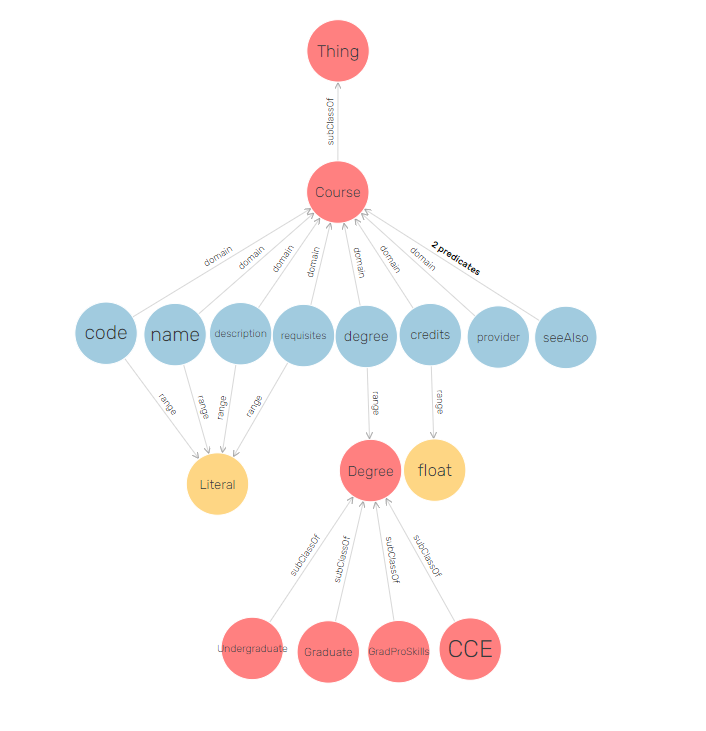
\includegraphics[width=3in]{img/course.png}
        \caption{Course Model.}
        \label{course_model}
        \end{figure}
  
        A \textit{Course} element defines a course offered at an Institute (see \textit{Fig. \ref{course_model}}). An instance of a \textit{Course} has a \textit{code}, \textit{name}, \textit{degree}, \textit{provider}, and a \textit{credit} attribute. Optional attributes, such as a \textit{description} and \textit{requisites}, may be provided as well.
        
        \begin{figure}[H]
        \centering
        
\includegraphics[width=1.5in]{img/course_instance.png}
        \caption{Course Instance.}
        \label{course_instance}
        \end{figure}
        
        In general, the \textit{code} defines the department associated with an instance of a \textit{Course}, as well as an identifier that is represented as a number. In \textit{Fig. \ref{course_instance}}, the code ACTU445 signifies that this \textit{Course} is found in the Department of Mathematics and Statistics and has been given a number of 256.
        
        The \textit{name} of a \textit{Course} is equivalent to its title and is represented as a string. In \textit{Fig. \ref{course_instance}}, the \textit{name} of this course is Mathematics of Finance.
        
        The \textit{description} attribute is an overview of a certain \textit{Course}, including the related concepts covered. In \textit{Fig. \ref{course_instance}}, the \textit{description} is found below the title. This attribute is optional as certain courses do not have descriptions tied to them.
        
        The \textit{degree} defines the level of education that an instance of a \textit{Course} belongs to. Not every course is limited to the undergraduate and/or graduate level. Some courses are also offered in more than one degree. For this reason, the \textit{degree} attribute is not restricted to being a primitive type.
        
        The \textit{credits} attribute defines the number of credits, represented as a floating point value, of a \textit{Course}. It may be that some courses offer no credits. This is generally found in courses offered in a workshop.
        
        The \textit{provider} of a \textit{Course} corresponds to the Institute that offers the course.
        
        The \textit{requisites} attribute defines enrolment requirements on a \textit{Course}. A course may be a pre-requisite or a co-requisite of some other course. As well, special permission by the department may be required to take a course. These details have been captured in \textit{Conupedia}, but not displayed. The reasoning behind this is that requisite expressions are written in the natural language, and are varied in their expressions. Advanced processing techniques are required to form these types of relations.
        
        Finally, the \textit{seeAlso} attribute defines the similarity relation between one course and another. A similarity relation is established based on the description of a \textit{Course}.

    \subsection{User}
        
        \begin{figure}[H]
        \centering
        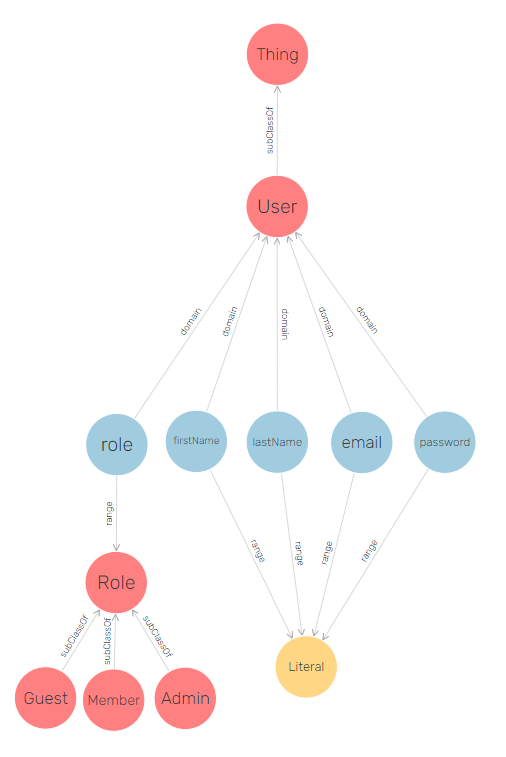
\includegraphics[width=2.0in]{img/user.png}
        \caption{User Model.}
        \label{user}
        \end{figure}
        
        
        The \textit{User} element defines the actors registered to the \textit{Conupedia} system (see \textit{Fig. \ref{user}}). An instance of this class contain attributes related to the person it belongs to, which includes, but is not limited to, their \textit{first} and \textit{last} names, \textit{email}, \textit{password}, and \textit{role}.
        
        While the \textit{email} attribute is used during the registration process to verify if an account already exists, and is used as part of the login field, we do not impose limitations on changing it at a later time. In fact, a different unique identifier is generated for every created instance of \textit{User}. This \textit{identifier} is used as part of the IRI that identifies a specific \textit{User}, and is mentioned in the \textit{identifier} property.\\
   
    \subsection{Rating}
        \begin{figure}[htpb]
        \centering
        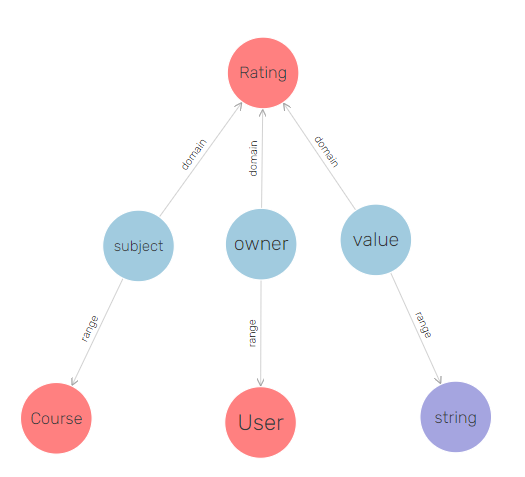
\includegraphics[width=2.0in]{img/rating.png}
        \caption{Rating Model.}
        \label{rating}
        \end{figure}
        
        User-course interactions are defined using the \textit{Rating} element (see \textit{Fig. \ref{rating}}). Every instance of a \textit{Rating} has an \textit{owner}, \textit{subject}, and \textit{value} attributes. The \textit{subject} and \textit{owner} of a \textit{Rating} points to the referable instances of a \textit{Course} and a \textit{User} respectively, while the \textit{value} defines the opinion expressed by the \textit{owner} on the \textit{subject}. 
        
        A user can express an opinion for some course. We assume that opinions are not influenced by other factors beyond reading of the title or description of any course. Using this assumption, we identify two main cases for user-course interactions. First, a user can express interest in some course. In \textit{Conupedia}, this opinion is represented using the like button. A user may also express dis-interest in some course. This opinion is represented using the dislike button. The assumption is that when users express interest in a course, they expect to receive content similar to that course. Similarly, when they express dis-interest in a course, then the expectation is that courses similar to the targeted course should not be displayed in the future.
              

  
\newpage
\section{Conupedia}
    \begin{figure}[H]
    \centering
    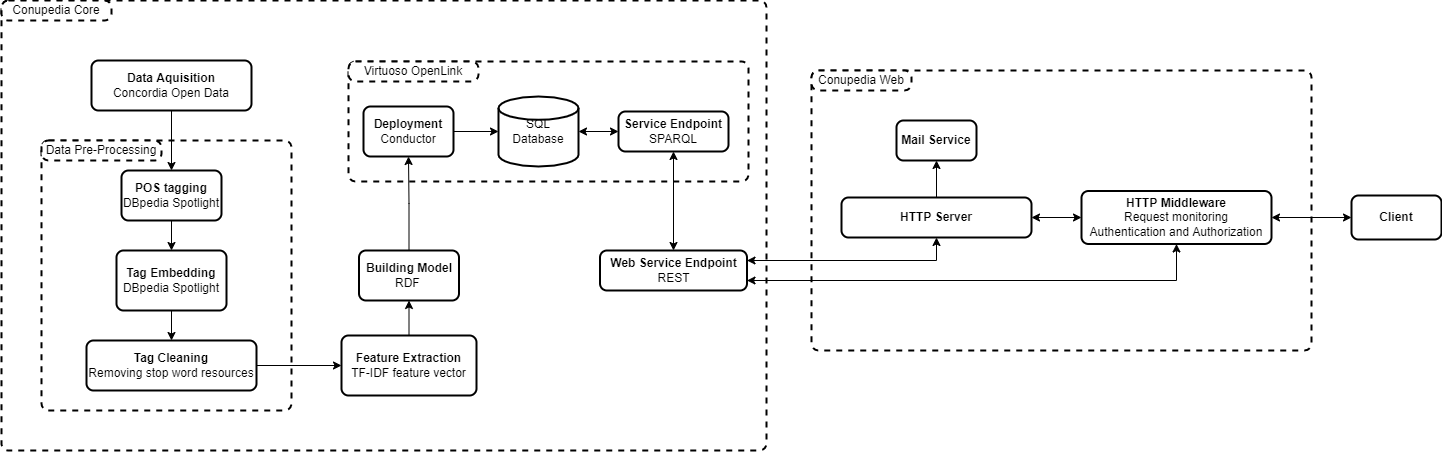
\includegraphics[width=3.25in]{img/architecture.png}
    \caption{Conupedia Application Design.}
    \label{conupedia_app}
    \end{figure}
    \textit{Conupedia} consists of two applications: \textit{Conupedia Core}, and \textit{Conupedia Web}.
    We distinguish the two applications by their functionalities, the cloud technology used, and the targeted audience (see \textit{Fig. \ref{conupedia_app}}).
    In this section, we elaborate on the proposed design, and the reasoning behind the distinction.
    
    \subsection{Conupedia Core}
        \textit{Conupedia Core} is a software for storing course related data remotely using cloud technologies.
        It is a SaaS that provides users with a web-based platform for uploading and maintaining course information without the hassles involved in maintaining a database.
        \textit{Conupedia Core} offers a number of features, such as the ability to track opinions expressed by users on courses, sorting of courses based on certain parameters (i.e popularity), and information pertaining to a given course (i.e degree level requirements).
        Users also benefit from the use of the built-in encryption techniques (i.e RS256) and hashing techniques (i.e SHA256) for securely storing customer information.
        \textit{Conupedia Core} is hosted on AWS for availability and scalability purposes.
        The underlying architecture consists of 2 main components: a database management, and web service endpoint.
        However, for demonstration purposes and as a proof of concept, we include 3 other components: data acquisition, data pre-processing, and feature extraction. \\
        
        \subsubsection{Data Aquisition}
        
           Open Data is a technology that collects information on various topics at Concordia University and transforms them into a machine-readable format \cite{b2}. 
            The information stored in Open Data is accessible via the application programming interface (API). 
            \textit{Conupedia} relies on this information to generate courses, along with their descriptions, codes, titles, and level of education. 
            The issue with Open Data, however, is that the information supplied is raw, with no context attached. 
            This means, data can be interpreted in a variety of ways, negatively impacting the results of \textit{Conupedia}'s recommendation engine.
            The data therefore needs to be pre-processed before being modelled.\\
            
            \subsubsection{Data Pre-Processing}
            A course description is an overview of the concepts related to a course.
            Terminologies found in descriptions can be abstract and/or specific and technical.
            The level of expressiveness in a description is generally proportional to its size.
            Course descriptions are also written in the natural language, and as such, there is an implicit assumption that the reader can extract context from these descriptions.
            In the data pre-processing stage, these concerns are addressed by proposing an approach to automating and enriching the tagging process of course descriptions.

            
            \begin{figure}[htbp]
            \centering
            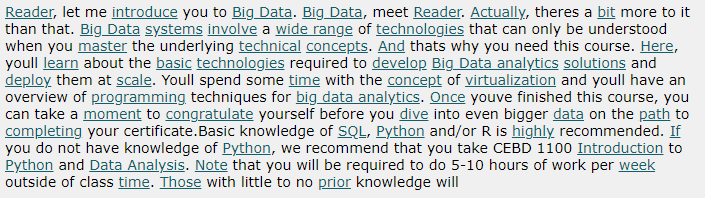
\includegraphics[width=3.5in]{img/dbpedia-spotlight.png}
            \caption{Automated Tagging using DBpedia Spotlight.}
            \label{fig_sim}
            \end{figure}

            
            The current solution relies on the use of an existing service called DBpedia Spotlight \cite{b3}.
            With this service, tags are extracted from natural language expressions by mapping them with existing resources found in the DBpedia data store.
            Since the same resource can be used in various domains and its interpretation depends on the context within which it is used in,  DBpedia Spotlight attempts to solve this problem by scoring each candidate resource according to its relatedness with the data provided.
            The extraction and relevancy of a resource is dependent on the user setting the confidence level appropriate to their use case.
            
            In \textit{Conupedia}, we use a confidence level of 0.35 to extract resources as it was observed to output the most relevant resources for descriptions containing abstract and specific terminologies.
            However, there still remained the issue of course descriptions that contained specific terminologies, and those that were abstract and small in size. 
            For example, consider a course containing a specific resource for \textit{Python}, and another for \textit{Programming Language}.
            This presents an issue when forming relations between the two courses as one of the resources is a specific instance of the other.
            There is also the problem of a course having few resources tied to it (i.e small or abstract), thus presenting a challenge when links are formed between it and other courses.
            
            \begin{figure}[htbp]
            \centering
            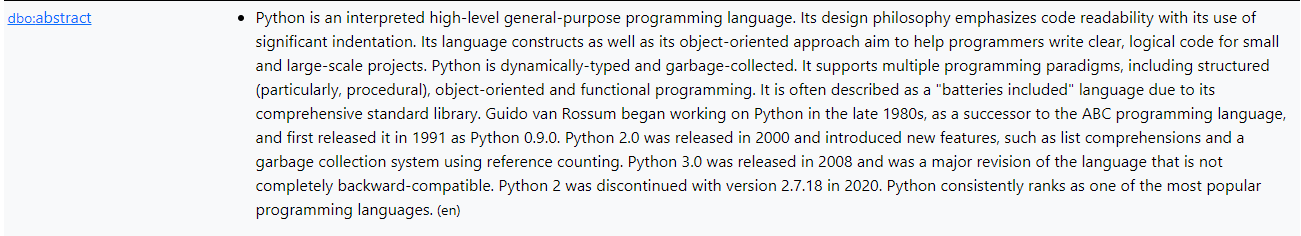
\includegraphics[width=3.5in]{img/python.png}
            \caption{Abstract Information in a DBpedia Resource}
            \label{abstract_info}
            \end{figure}
            
            Abstract information related to the outputs of DBpedia Spotlight are also taken into consideration in the \textit{Conupedia} system (see \textit{Fig. \ref{abstract_info}}).
            These pieces of information are fed back into DBpedia Spotlight as input and the outputs are used to enrich the set of resources tied to a course.
            Thresholds are used to constraint the number of resources bound to courses, and the maximum depth allowable while extracting resources.
            
            With a confidence level of 0.35, undesirable resources can be extracted from course descriptions. 
            For example, the \textit{This} resource does not participate in describing concepts of a course.
            \textit{Conupedia} eliminates these types of resources by referring to the corpus of common English stop words in the \textit{sklearn} module \cite{b6}.
            The remaining resources bound to courses are converted to tags and used in the feature extraction stage.\\

        \subsubsection{Feature Extraction}
        

            To generate a match rate for all courses, we considered the tags belonging to every course.
            These tags were fitted onto a term frequency-inverse document frequency feature matrix using \textit{sklearn}.
            The motivation behind using a TF-IDF feature matrix is to reduce the weight of terms that were common in all descriptions, while increasing the weight of those that were specific to some courses.
            The match rate was computed using the cosine similarity of the TF-IDF matrix.
            \begin{figure}[H]
            \centering
            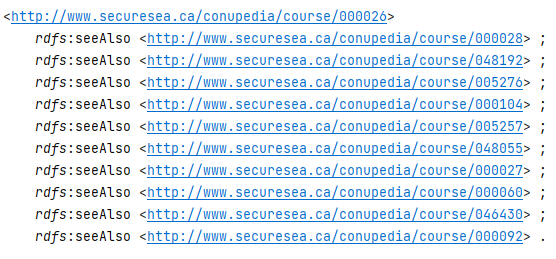
\includegraphics[width=3.0in]{img/top10.png}
            \caption{Course Match Expression.}
            \label{top10}
            \end{figure}
            In \textit{Fig. \ref{top10}}, an instance of a \textit{Course} is linked to other \textit{Courses} based on the top 10 highest match rates. These references are queried when producing a list of recommendations. We note that not all courses in the list are displayed as it depends on whether or not the user has previously seen them. \\
            
        \subsubsection{Database Management}
            In Conupedia, the knowledge base is stored and managed by the Virtuoso OpenLink database manager.
            Administration tasks, such as importing and exporting the data store, are performed using the Conductor plugin.
            Data in store can be queried and modified via Virtuoso's built-in SPARQL endpoint.\\
            
            
        \subsubsection{Web Service Endpoint}
            While the SPARQL endpoint allows for REST calls to be made to it, we determined that having a REST API specific to the use cases studied in Conupedia was more appropriate for operating the database system. 
            In this way, the technicalities for manipulating data can be abstracted and make it so that it is friendly for the user making the calls.
            
            \newpage
            \begin{table}[H]
                \caption{Conupedia Core Web Service REST API}
                \begin{center}
                    \begin{tabular}{|c|c|c|}
                        \hline
                        \textbf{Resource}& \multicolumn{2}{|c|}{\textbf{Exposed subset of the uniform interface}}\\
                        \cline{2-3} 
                        \textbf{} & \textbf{\textit{Operation}}& \textbf{\textit{HTTP Action}}\\
                        \cline{1-3} 
                        \textbf{Course} & \textbf{\textit{List courses}}& \textbf{\textit{GET /courses }}\\
                        \textbf{} & \textbf{\textit{List courses by category}}& \textbf{\textit{GET /courses?category=\{key$^{\mathrm{a}}$\} }}\\
                        \textbf{} & \textbf{\textit{Create new course}}& \textbf{\textit{POST /courses }}\\
                        \textbf{} & \textbf{\textit{Read course information}}& \textbf{\textit{GET /courses/\{id\} }}\\
                        \textbf{} & \textbf{\textit{Delete course}}& \textbf{\textit{DELETE /courses/\{id\} }}\\
                        \textbf{} & \textbf{\textit{Update existing course}}& \textbf{\textit{PATCH /courses/\{id\} }}\\
                        
                        \cline{1-3}
                        \textbf{User} & \textbf{\textit{List users}}& \textbf{\textit{GET /users }}\\
                        \textbf{} & \textbf{\textit{List users by key}}& \textbf{\textit{GET /users?\{key$^{\mathrm{b}}$\}=\{value\} }}\\
                        \textbf{} & \textbf{\textit{Create new user}}& \textbf{\textit{POST /users }}\\
                        \textbf{} & \textbf{\textit{Read user information}}& \textbf{\textit{GET /users/\{id\} }}\\
                        \textbf{} & \textbf{\textit{Delete user}}& \textbf{\textit{DELETE /users/\{id\} }}\\
                        \textbf{} & \textbf{\textit{Update existing user}}& \textbf{\textit{PATCH /users/\{id\} }}\\
                        
                        \cline{1-3}
                        \textbf{Rating} & \textbf{\textit{List ratings}}& \textbf{\textit{GET /ratings }}\\
                        \textbf{} & \textbf{\textit{List ratings by key}}& \textbf{\textit{GET /ratings?\{key$^{\mathrm{c}}$\}=\{value\} }}\\
                        \textbf{} & \textbf{\textit{Create new rating}}& \textbf{\textit{POST /ratings }}\\
                        \textbf{} & \textbf{\textit{Read rating information}}& \textbf{\textit{GET /ratings/\{id\} }}\\
                        \textbf{} & \textbf{\textit{Delete rating}}& \textbf{\textit{DELETE /ratings/\{id\} }}\\
                        \textbf{} & \textbf{\textit{Update existing rating}}& \textbf{\textit{PATCH /ratings/\{id\} }}\\
                        
                        \hline
                        
                        \multicolumn{3}{l}{$^{\mathrm{a}}$key is one of latest, explore, popular, recommendations, likes}\\
                        \multicolumn{3}{l}{$^{\mathrm{b}}$key is one of id, first name, last name, email, password, role}\\
                        \multicolumn{3}{l}{$^{\mathrm{c}}$key is one of id, owner, subject, value}
                    \end{tabular}
                \label{tab1}
                \end{center}
            \end{table}
            
            The capabilities of the \textit{Conupedia Core} software includes the ability to create, modify, and query \textit{Users}, \textit{Courses}, and \textit{Ratings} (see \textit{Table \ref{tab1}}). Here, the intention is that users can implement their own flavors of course-recommendation systems without having to re-configure the back-end system or incur limitations in storage and computing.
            
    \subsection{Conupedia Web}
        \textit{Conupedia Web} is a web application that makes it easy for end-users to explore various courses offered by an Institute.
        Users who sign-up to the website can interact with courses and acquire recommendations based on their interactions.
        \textit{Conupedia Web} is dependant on \textit{Conupedia Core} and its features to provide various functionalities in a user-friendly way.
        It is defined as a flavor of a course-recommendation system for Concordia University, and can be hosted using any PaaS provider.
        For the purposes of this demonstration and as proof of concept, we present two main components of \textit{Conupedia Web}: an HTTP middleware, and an HTTP server.\\
        
        \subsubsection{HTTP Middleware}
            The HTTP middleware component of \textit{Conupedia Web} intercepts all incoming requests from the web server endpoint and verifies their authenticity.
            A request is authentic if information contained in the session cookie can be decrypted and mapped to an existing user.
            When a user logs in to \textit{Conupedia}, their information is encrypted using a private key and sent back to the user using the \textit{set-cookie} http header.
            Throughout a given session, the information stored in the cookie is used to determine if it belongs to a valid user.
            In the case where it is valid, the \textit{HTTP middleware} component forwards the request to the main \textit{HTTP server}, where it is further processed.
            The response from the \textit{HTTP server} is then forwarded back to the user.
            However, if a request is not valid, the client is requested to remove the cookie and is redirected to the login page. 
            
        
        \subsubsection{HTTP Server}
            The \textit{HTTP server} component processes incoming requests from the \textit{HTTP middleware}.
            It's primary purpose is to handle several types of requests by referring to information stored in \textit{Conupedia Core}.
            
            \begin{table}[H]
                \caption{Conupedia Web Service REST API}
                \begin{center}
                \begin{tabular}{|c|c|c|}
                \hline
                \textbf{Resource}& \multicolumn{2}{|c|}{\textbf{Exposed subset of the uniform interface}}\\
                \cline{2-3} 
                \textbf{} & \textbf{\textit{Operation}}& \textbf{\textit{HTTP Action}}\\
                \cline{1-3} 
                \textbf{Public} & \textbf{\textit{Show log in}}& \textbf{\textit{GET /login }}\\
                \textbf{} & \textbf{\textit{Show sign up}}& \textbf{\textit{GET /register }}\\
                \textbf{} & \textbf{\textit{Submit log in details}}& \textbf{\textit{POST /login }}\\
                \textbf{} & \textbf{\textit{Submit sign up details}}& \textbf{\textit{POST /register }}\\
                \textbf{} & \textbf{\textit{Activate account}}& \textbf{\textit{GET /activate?id=\{code$^{\mathrm{a}}$\} }}\\
                \cline{1-3} 
                \textbf{Protected} & \textbf{\textit{Show main page}}& \textbf{\textit{GET / }}\\
                \textbf{} & \textbf{\textit{Log out}}& \textbf{\textit{GET /logout }}\\
                \textbf{} & \textbf{\textit{Show account settings}}& \textbf{\textit{GET /setting }}\\
                \textbf{} & \textbf{\textit{Change account settings}}& \textbf{\textit{POST /setting }}\\
                \hline
                \multicolumn{3}{l}{$^{\mathrm{a}}$code is provided by email}\\
                \end{tabular}
                \label{tab2}
                \end{center}
            \end{table}
        
    
            API calls are classified into two categories: public, and protected (see \textit{Table \ref{tab2}}).
            Protected calls cannot be accessed without authentication.
            This is granted when the user sends a valid POST request in the log in page.
            
            
            \begin{figure}[htbp]
            \centering
            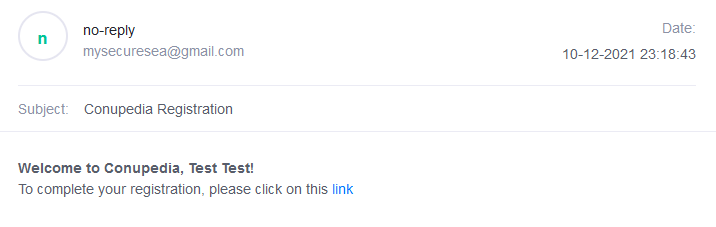
\includegraphics[width=3.0in]{img/email.png}
            \caption{Email Activation Message.}
            \label{email}
            \end{figure}
            
            
            Anyone can sign up by filling out their details in the register page.
            When the form is submitted, the server verifies the email address of the user against an existing entry in the database system.
            If the provisioned email address already exists, the user needs to supply another address.
            Otherwise, the account is created and an activation message is sent via email (see \textit{Fig. \ref{email}}).
            
            \begin{figure}[H]
            \centering
            
\includegraphics[width=1.5in]{img/course_interaction.png}
            \caption{Course Interaction Options.}
            \label{course_interaction}
            \end{figure}
            
            When a user logs in to \textit{Conupedia}, they are directed to the \textit{Explore} section within the root directory.
            The user is presented with a list of courses.
            An interaction from a user involves either liking or disliking a certain course.
            This is achieved by hovering over a course, and selecting the appropriate reaction (see \textit{Fig. \ref{course_interaction}}).
            
            
            \begin{figure}[H]
            \centering
            
\includegraphics[width=3.0in]{img/headline.png}
            \caption{Course Categories.}
            \label{headline}
            \end{figure}
            
            A user can also visit other categories.
            To date, \textit{Conupedia} supports the display of courses in the recommendations, latest, likes, and popular categories (see \textit{Fig. \ref{headline}}).
            
            \begin{figure}[htbp]
            \centering
            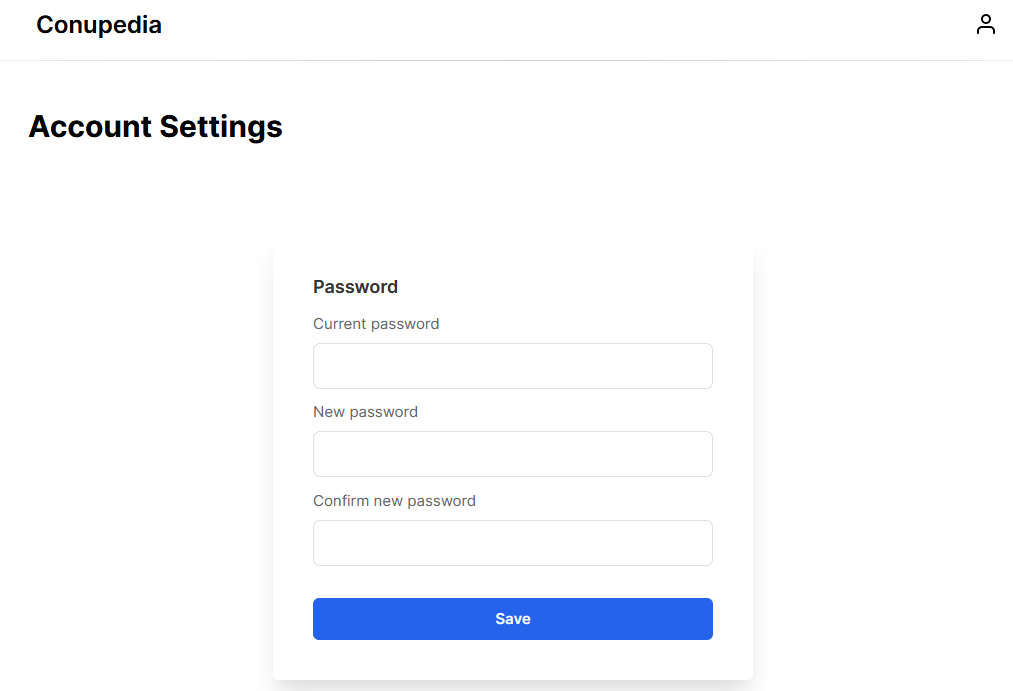
\includegraphics[width=3.0in]{img/password.png}
            \caption{Account Settings.}
            \label{setting}
            \end{figure}
            
            Finally, a user can access the settings page, where they can request for a new password (see \textit{Fig. \ref{setting}}).
            The server verifies the current password of a user by matching it with the related entry in the database system.
            If a match is found, the password is updated.
            
            Indeed, the main purpose of the web server in \textit{Conupedia} is to present information supplied by the database system in a human-friendly manner by hiding the underlying technicalities involved in communication.
            The server also monitors for ill-formed, or invalid requests on resources by preventing them from reaching the database system.
    

\section{Conclusion}
    Persistent modifications of entries within the course calendar at Concordia University necessitates students to consult these changes and to adapt their existing scheduling plan when a conflict occurs.
    Conflicts may also not be detected until a student is given access to the enrolment cart during the registration period.
    For this reason, we propose \textit{Conupedia}.
    This system adapts to changes in the availability of courses in an autonomous manner and provides users with course recommendations that are personalized to their interest and requirements.



\begin{thebibliography}{00}
    \bibitem{b1} ``Conupedia,'' Accessed on: Dec. 15, 2021. [Online]. Available: \url{http://securesea.ca/}
    
    \bibitem{b2} ``Concordia's Open Data,'' Accessed on: Oct. 15, 2021. [Online]. Available: \url{https://www.concordia.ca/web/open-data.html}
    
    \bibitem{b3}  ``DBpedia Spotlight,'' Accessed on: Oct. 15, 2021. [Online]. Available: \url{https://www.dbpedia-spotlight.org/}
    
    \bibitem{b4}  ``Virtuoso OpenLink Documentation,'' Accessed on: Oct. 15, 2021. [Online]. Available: \url{http://docs.openlinksw.com/virtuoso/}
    
    \bibitem{b5}  ``Ontotext GraphDB Documentation,'' Accessed on: Oct. 15, 2021. [Online]. Available: \url{https://graphdb.ontotext.com/documentation/standard/}
    
    \bibitem{b6}  ``Scikit Learn - User Guide,'' Accessed on: Oct. 15, 2021. [Online]. Available: \url{https://scikit-learn.org/stable/user_guide.html}
\end{thebibliography}
\vspace{12pt}

\end{document}
